\documentclass[aspectratio=169]{beamer}
\usepackage[utf8]{inputenc}

\usetheme{Madrid}
\usefonttheme[onlymath]{serif}

\AtBeginSection[]{
  \begin{frame}
  \vfill
  \centering
  \begin{beamercolorbox}[sep=8pt,center,shadow=true,rounded=true]{title}
    \usebeamerfont{title}\insertsectionhead\par%
  \end{beamercolorbox}
  \vfill
  \end{frame}
}

\usepackage{amsmath}
\usepackage{amssymb}
\usepackage{bm}

\renewcommand{\Vec}[1]{\bm{#1}}
\newcommand{\Mat}[1]{\mathbf{#1}}
\newcommand{\Tns}[1]{\mathcal{#1}}

\newcommand{\D}{\,\mathrm{d}}

\newcommand{\Ord}{\mathcal{O}}

\newcommand{\RR}{\mathbb{R}}

\usepackage{algpseudocode}

\usepackage{graphicx}
\usepackage{tikz}
\usetikzlibrary{arrows.meta}

\title{Tensor Train Decomposition}
\author{Saibal De}
\date{October 27, 2020}

\begin{document}

\begin{frame}
    \titlepage
\end{frame}

\section{Tensors}

\begin{frame}{Definition}
  \begin{itemize}
    \item
      Formally, element from product of abstract vector spaces
    \item
      For our purposes, a multi-dimensional array
      \begin{equation*}
        \Tns{X} \in \RR^{n_1 \times \cdots \times n_d}
      \end{equation*}
    \item
      Elements are indexed by
      \begin{equation*}
        \Tns{X}(i_1, \ldots, i_d), \quad 1 \leq i_k \leq n_k, \quad 1 \leq k
        \leq d
      \end{equation*}
    \item
      Special cases:
      \begin{itemize}
        \item
          $d = 0$: Scalar $x$
        \item
          $d = 1$: Vector $\Vec{x}$
        \item
          $d = 2$: Matrix $\Mat{X}$
      \end{itemize}
  \end{itemize}
\end{frame}

\begin{frame}{Applications}
  \begin{itemize}
    \item
      A lot of data is naturally multi-dimensional, e.g., videos
    \item
      Scientific simulation outputs are often high-dimensional tensors
    \item
      Why do we care in a fast algorithms class?
  \end{itemize}
\end{frame}

\section{Motivation}

\begin{frame}{Integral Equations}
  \begin{itemize}
    \item
      Laplace equation $-\Delta u = 0$ in domain $\Omega \in \RR^2$
    \item
      Green's function
      \begin{equation*}
        k(\Vec{x}, \Vec{y}) = -\frac{1}{2\pi} \log{\lvert \Vec{x} - \Vec{y}
        \rvert}
      \end{equation*}
    \item
      Construct solution by integrating over boundary $\Gamma = \partial\Omega$
      \begin{equation*}
        u(\Vec{x}) = \int_\Gamma k(\Vec{x}, \Vec{y}) \sigma(\Vec{y})
        \D\Gamma(\Vec{y})
      \end{equation*}
    \item
      Enforce boundary condition $u = f$ on boundary $\Gamma$
      \begin{equation*}
        \int_\Gamma k(\Vec{x}, \Vec{y}) \sigma(\Vec{y}) \D\Gamma(\Vec{y}) =
        f(\Vec{x}), \quad \Vec{x} \in \Gamma
      \end{equation*}
      and solve for unknown $\sigma$
  \end{itemize}
\end{frame}

\begin{frame}{Nystr\"om Discretization}
  \begin{itemize}
    \item
      Consider the simplified problem
      \begin{equation*}
        \int_0^1 k(x, y) \sigma(y) \D{y} = f(x), \quad x \in [0, 1]
      \end{equation*}
      with smoothed kernel $k(x, y) = -\log{(\lvert x - y \rvert + \epsilon)}$
    \item
      Choose discretization points $x_i = \frac{i}{N - 1}$, $0 \leq i \leq N -
      1$
    \item
      Discretized equation
      \begin{equation*}
        \Mat{K} \Vec{\sigma} = \Vec{f}, \quad K_{ij} = k(x_i - x_j), \quad
        \sigma_j = \sigma(x_j), \quad f_i = f(x_i)
      \end{equation*}
    \item
      Iterative methods: Need fast $\Vec{\sigma} \mapsto \Mat{K} \Vec{\sigma}$
      implementation
  \end{itemize}
\end{frame}

\begin{frame}{Low-Rank Factorization}
  \begin{itemize}
    \item
      Given kernel matrix $\Mat{K} \in \RR^{N \times N}$, factorize
      \begin{equation*}
        \Mat{K} = \Mat{A} \Mat{B}^\top, \quad \Mat{A}, \Mat{B} \in \RR^{N \times
        r}
      \end{equation*}
    \item
      Multiplying $\Mat{K} \Vec{\sigma}$ takes $\Ord(N r)$ operations
    \item
      Unfortunately, $\Mat{K}$ is full rank, $r = N$
  \end{itemize}
\end{frame}

\begin{frame}{Kernel Matrix}
  \centering
  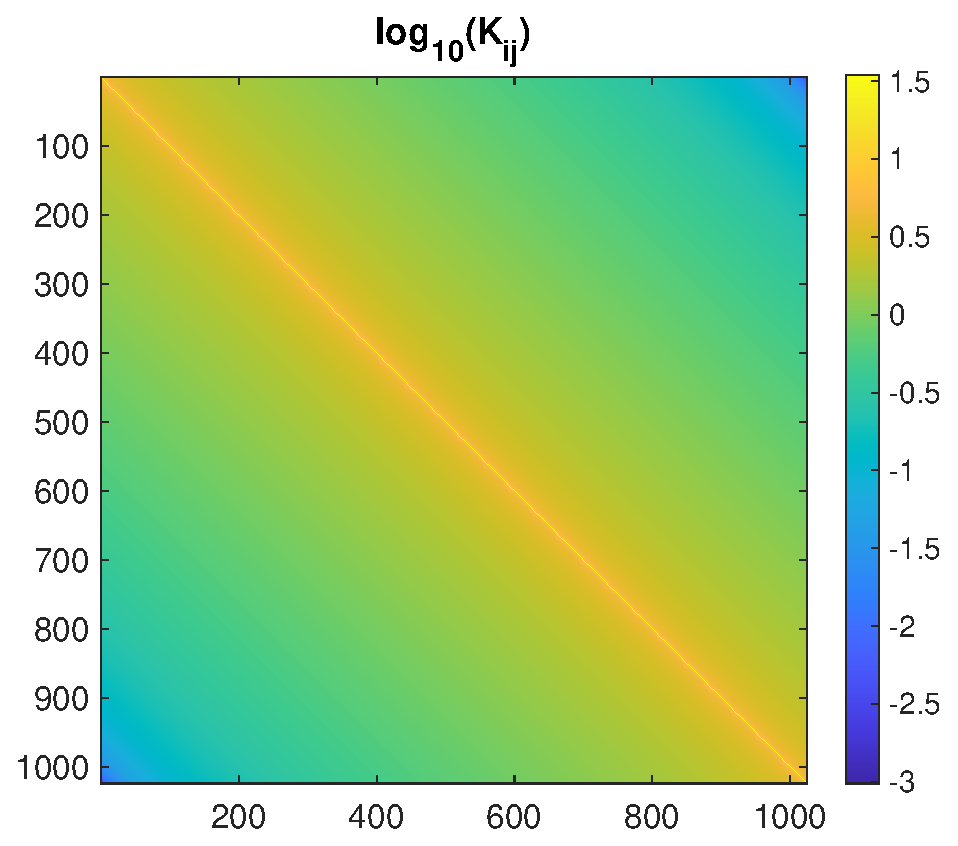
\includegraphics[width=0.45\textwidth]{../figures/kernel_magnitude.eps}
\end{frame}

\begin{frame}{Hierarchical Kernel Factorization}
  \centering
  \begin{minipage}{0.45\textwidth}
    \centering
    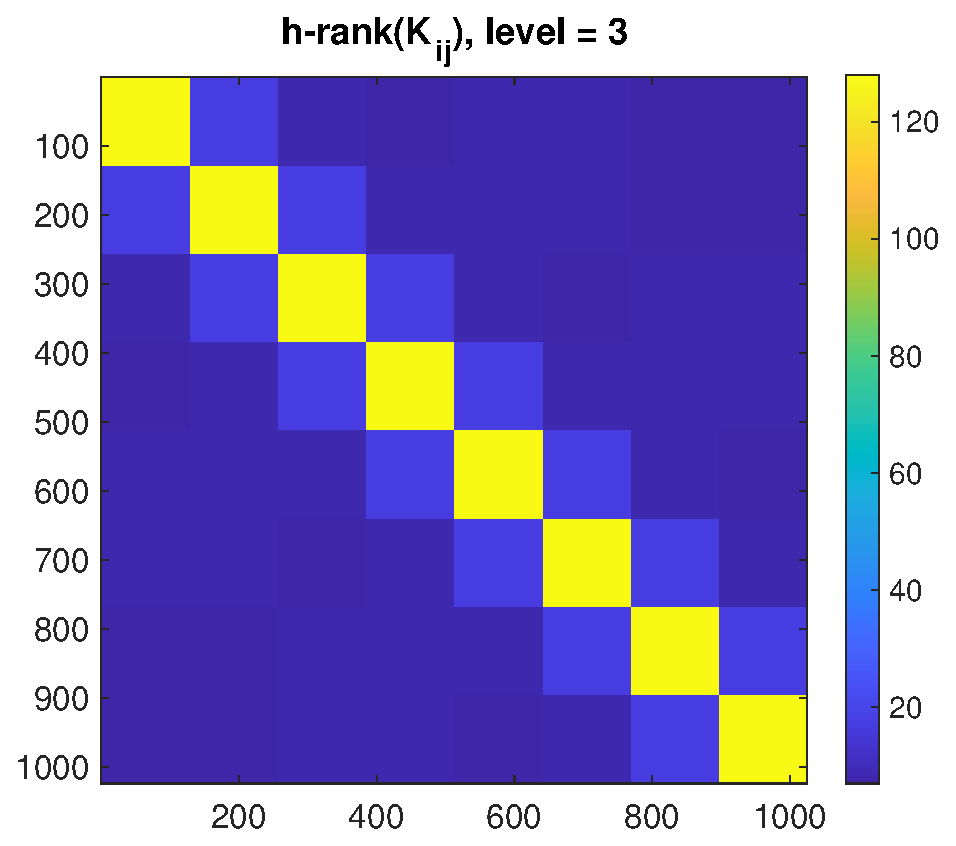
\includegraphics[width=\linewidth]{../figures/kernel_h_rank_3.eps}
  \end{minipage}
  ~
  \begin{minipage}{0.45\textwidth}
    \centering
    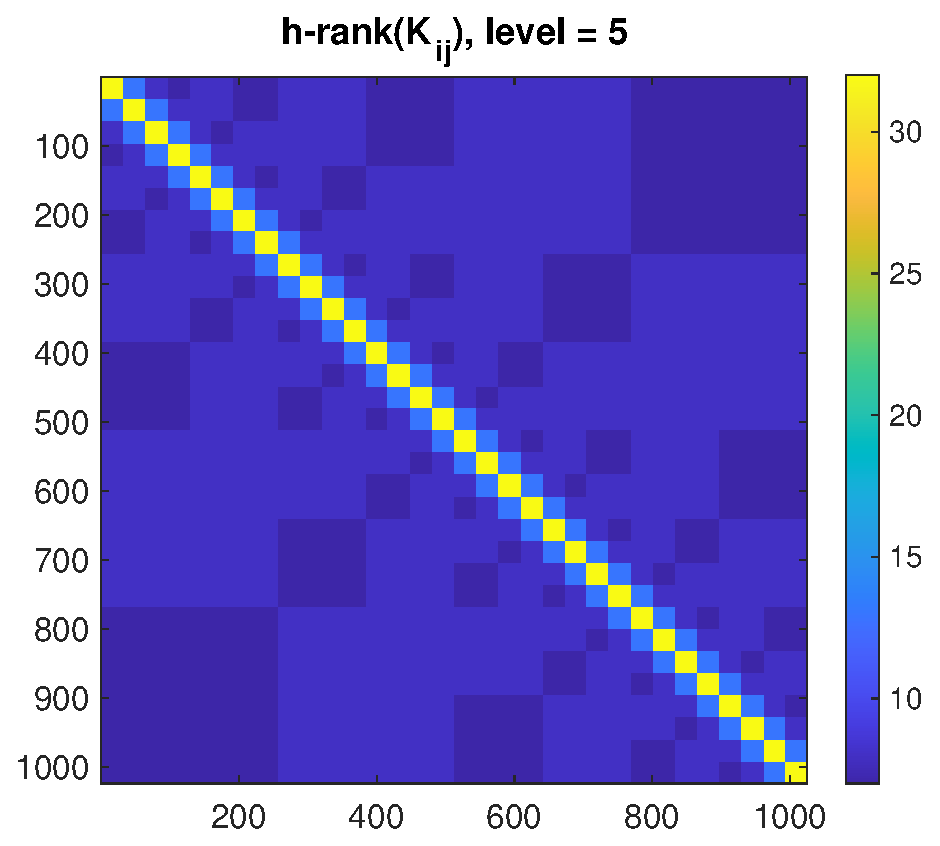
\includegraphics[width=\linewidth]{../figures/kernel_h_rank_5.eps}
  \end{minipage}
\end{frame}

\begin{frame}{Hierarchical Domain Decomposition}
  \centering
  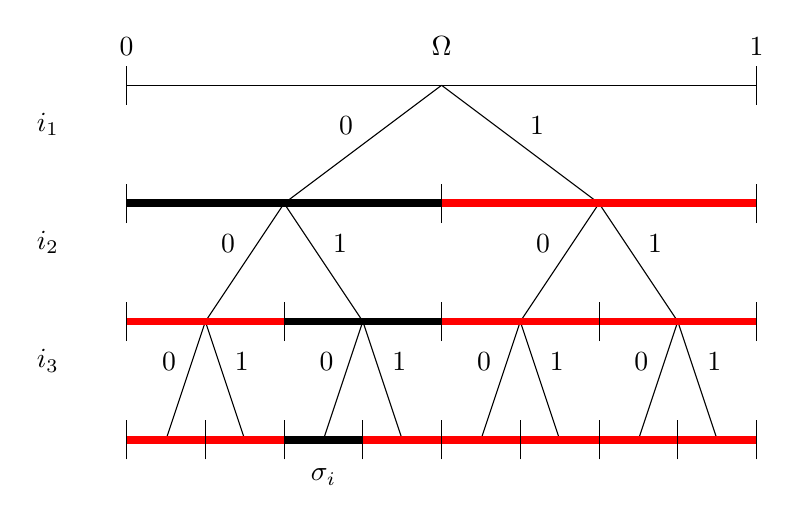
\begin{tikzpicture}
    \draw (4.0, 4.5) -- node [anchor=south east] {$0$} (2.0, 3.0);
    \draw (4.0, 4.5) -- node [anchor=south west] {$1$} (6.0, 3.0);

    \draw (2.0, 3.0) -- node [anchor=south east] {$0$} (1.0, 1.5);
    \draw (2.0, 3.0) -- node [anchor=south west] {$1$} (3.0, 1.5);
    \draw (6.0, 3.0) -- node [anchor=south east] {$0$} (5.0, 1.5);
    \draw (6.0, 3.0) -- node [anchor=south west] {$1$} (7.0, 1.5);

    \draw (1.0, 1.5) -- node [anchor=south east] {$0$} (0.5, 0.0);
    \draw (1.0, 1.5) -- node [anchor=south west] {$1$} (1.5, 0.0);
    \draw (3.0, 1.5) -- node [anchor=south east] {$0$} (2.5, 0.0);
    \draw (3.0, 1.5) -- node [anchor=south west] {$1$} (3.5, 0.0);
    \draw (5.0, 1.5) -- node [anchor=south east] {$0$} (4.5, 0.0);
    \draw (5.0, 1.5) -- node [anchor=south west] {$1$} (5.5, 0.0);
    \draw (7.0, 1.5) -- node [anchor=south east] {$0$} (6.5, 0.0);
    \draw (7.0, 1.5) -- node [anchor=south west] {$1$} (7.5, 0.0);

    \draw (0.0, 4.5) -- (8.0, 4.5);
    \foreach \x in {0, 8} {
      \draw (\x, 4.25) -- (\x, 4.75);
    }
    \node [anchor=south] at (0.0, 4.75) {$0$};
    \node [anchor=south] at (4.0, 4.75) {$\Omega$};
    \node [anchor=south] at (8.0, 4.75) {$1$};

    \draw [line width=1mm, red] (0.0, 3.0) -- (8.0, 3.0);
    \draw [line width=1mm] (0.0, 3.0) -- (4.0, 3.0);
    \node at (-1.0, 4.0) {$i_1$};
    \foreach \x in {0, 4, 8} {
      \draw (\x, 2.75) -- (\x, 3.25);
    }

    \draw [line width=1mm, red] (0.0, 1.5) -- (8.0, 1.5);
    \draw [line width=1mm] (2.0, 1.5) -- (4.0, 1.5);
    \node at (-1.0, 2.5) {$i_2$};
    \foreach \x in {0, 2, 4, 6, 8} {
      \draw (\x, 1.25) -- (\x, 1.75);
    }

    \draw [line width=1mm, red] (0.0, 0.0) -- (8.0, 0.0);
    \draw [line width=1mm] (2.0, 0.0) -- (3.0, 0.0);
    \node at (-1.0, 1.0) {$i_3$};
    \foreach \x in {0, 1, 2, 3, 4, 5, 6, 7, 8} {
      \draw (\x, -0.25) -- (\x, 0.25);
    }

    \node [anchor=north] at (2.5, -0.25) {$\sigma_i$};
  \end{tikzpicture}
\end{frame}

\begin{frame}{Tensorization/Vectorization}
  \centering
  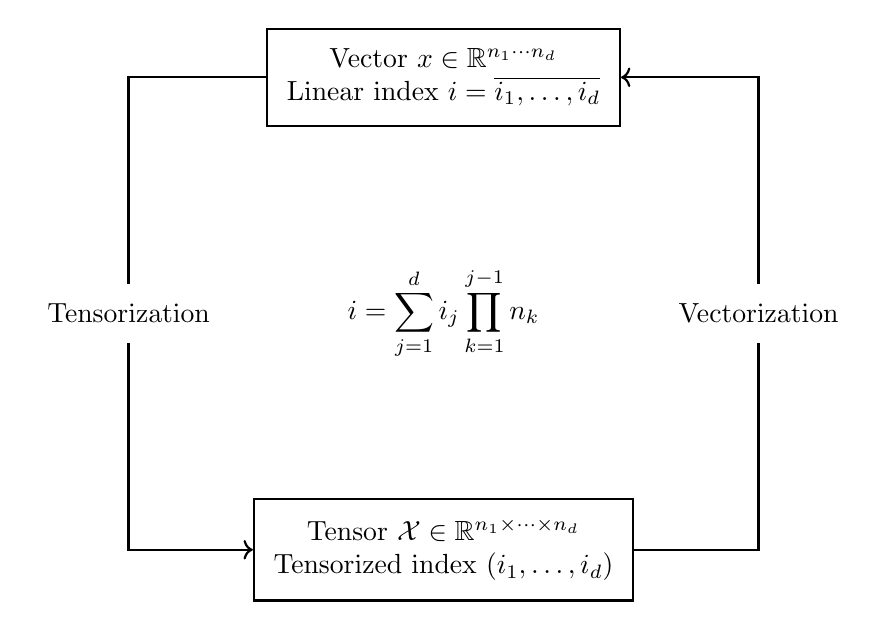
\begin{tikzpicture}
    \node [thick, draw, inner sep=0.25cm, align=center] (V) at (0,  3) {%
      Vector $x \in \mathbb{R}^{n_1 \cdots n_d}$ \\
      Linear index $i = \overline{i_1, \ldots, i_d}$
    };
    \node [thick, draw, inner sep=0.25cm, align=center] (T) at (0, -3) {%
      Tensor $\mathcal{X} \in \mathbb{R}^{n_1 \times \cdots \times n_d}$ \\
      Tensorized index $(i_1, \ldots, i_d)$
    };
    \node at (0,  0) {%
      $i = \displaystyle\sum_{j = 1}^d i_j \displaystyle\prod_{k = 1}^{j - 1}
      n_k$
    };
    \draw [thick, ->] (V.west) -- (-4,  3) -- 
        node [thick, fill=white, inner sep=0.25cm] {Tensorization} (-4, -3) --
        (T.west);
    \draw [thick, ->] (T.east) -- ( 4, -3) --
        node [thick, fill=white, inner sep=0.25cm] {Vectorization} ( 4,  3) --
        (V.east);
  \end{tikzpicture}
\end{frame}

\section{Tensor Train Format}

\begin{frame}{Challenges in Tensor Computations}
  \begin{itemize}
    \item
      Tensor $\Tns{X} \in \RR^{n_1 \times \cdots \times n_d}$
    \item
      Storing all entries requires $\Ord(n^d)$ memory, $n = \max\{n_1, \ldots,
      n_d\}$
    \item
      Any operation involving full tensors has complexity $\Ord(n^d)$
    \item
      Impractical in high dimensions: "Curse of dimensionality"
    \item
      Can we do better?
  \end{itemize}
\end{frame}

\begin{frame}{Motivation: Low-Rank Matrix Factorization}
  \begin{itemize}
    \item
      Matrix factorization $\Mat{X} = \Mat{A} \Mat{B}$, $\Mat{A} \in \RR^{m
      \times r}$, $\Mat{B} \in \RR^{r \times n}$
    \item
      Elements
      \begin{equation*}
        \begin{split}
          \Mat{X}(i_1, i_2)
          &= \Mat{A}(i_1, :) \Mat{B}(:, i_2) \qquad \text{MATLAB Notation} \\
          &= \underbrace{\Mat{A}(i_1)}_{1 \times r} \underbrace{\Mat{B}(i_2)}_{r
          \times 1} \,\quad\qquad \text{Simplified Notation}
        \end{split}
      \end{equation*}
    \item
      Generalize
      \begin{equation*}
        \Tns{X}(i_1, i_2, \ldots, i_d) = \underbrace{\Mat{X}_1(i_1)}_{r_0 \times
        r_1} \underbrace{\Mat{X}_2(i_2)}_{r_1 \times r_2} \cdots
        \underbrace{\Mat{X}_d(i_d)}_{r_{d - 1} \times r_d}, \quad r_0 = r_d = 1
      \end{equation*}
  \end{itemize}
\end{frame}

\begin{frame}{Format Definition}
  \begin{itemize}
    \item
      Tensor-train (TT) format
      \begin{equation*}
        \Tns{X}(i_1, i_2, \ldots, i_d) = \underbrace{\Mat{X}_1(i_1)}_{r_0 \times
        r_1} \underbrace{\Mat{X}_2(i_2)}_{r_1 \times r_2} \cdots
        \underbrace{\Mat{X}_d(i_d)}_{r_{d - 1} \times r_d}, \quad r_0 = r_d = 1
      \end{equation*}
    \item
      Expanding the matrix products
      \begin{equation*}
        \Tns{X}(i_1, i_2, \ldots, i_d) = \sum_{\alpha_0 = 1}^{r_0}
        \sum_{\alpha_1 = 1}^{r_1} \cdots \sum_{\alpha_d = 1}^{r_d}
        \Tns{X}_1(\alpha_0, i_1, \alpha_1) \Tns{X}_2(\alpha_1, i_2, \alpha_2)
        \cdots \Tns{X}_d(\alpha_{d - 1}, i_d, \alpha_d)
      \end{equation*}
    \item
      Storage costs $\Ord(\sum_{k = 1}^d r_{k - 1} n_k r_k) = \Ord(d n r^2)$
      with $r = \max\{r_1, \ldots, r_{d - 1}\}$
    \item
      Evaluation of any entry costs $\Ord(d r^2)$
  \end{itemize}
\end{frame}

\begin{frame}{Terminology}
  \begin{itemize}
    \item
      TT ranks $r_1, \ldots, r_{d - 1}$
    \item
      Maximal TT rank $r = \max\{r_1, \ldots, r_{d - 1}\}$
    \item
      TT cores $\Tns{X}_1, \ldots, \Tns{X}_d$
  \end{itemize}
\end{frame}

\begin{frame}{Examples}
  \begin{itemize}
    \item
      Sometimes we can construct the TT decomposition analytically
    \item
      $\Tns{X}(i_1, \ldots, i_d) = i_1 + \cdots + i_d$
      \begin{equation*}
        \Mat{X}_1(i_1) =
        \begin{bmatrix}
          i_1 & 1
        \end{bmatrix},
        \quad \Mat{X}_k(i_k) =
        \begin{bmatrix}
          1 & 0 \\
          i_k &  1
        \end{bmatrix},
        \quad \Mat{X}_d(i_d) =
        \begin{bmatrix}
          1 \\
          i_d
        \end{bmatrix}
      \end{equation*}
    \item
      $\Tns{X}(i_1, \ldots, i_d) = \sin(i_1 + \cdots + i_d)$
      \begin{equation*}
        \Mat{X}_1(i_1) =
        \begin{bmatrix}
          \sin i_1 & \cos i_1
        \end{bmatrix},
        \quad \Mat{X}_k(i_k) =
        \begin{bmatrix}
          \cos i_k & -\sin i_k \\
          \sin i_k &  \cos i_k
        \end{bmatrix},
        \quad \Mat{X}_d(i_d) =
        \begin{bmatrix}
          \cos i_d \\
          \sin i_d
        \end{bmatrix}
      \end{equation*}
  \end{itemize}
\end{frame}

\begin{frame}{Questions}
  \begin{itemize}
    \item
      How big can maximal TT rank $r$ can become?
    \item
      How do we compute TT decomposition?
    \item
      Are there any advantages other than storage?
  \end{itemize}
\end{frame}

\section{Fast Operations in TT Format}

\begin{frame}{Premise}
  \begin{itemize}
    \item
      Tensors $\Tns{X}$ and $\Tns{Y}$ of size $n_1 \times \cdots \times n_d$
    \item
      TT decompositions
      \begin{align*}
        \Tns{X}(i_1, \ldots, i_d) &= \Mat{X}_1(i_1) \cdots \Mat{X}_d(i_d) \\
        \Tns{Y}(i_1, \ldots, i_d) &= \Mat{Y}_1(i_1) \cdots \Mat{Y}_d(i_d)
      \end{align*}
    \item
      Can we efficiently perform linear algebra operations in TT format?
    \item
      I.\ V.\ Oseledets (2011). \textit{Tensor-train decomposition.} SIAM
      Journal on Scientific Computing.
  \end{itemize}
\end{frame}

\begin{frame}{Tensor Sum}
  \begin{itemize}
    \item
      Cores of tensor sum $\Tns{Z} = \Tns{X} + \Tns{Y}$ can be computed as
      \begin{align*}
        \Mat{Z}_1(i_1) &=
        \begin{bmatrix}
          \Mat{X}_1(i_1) & \Mat{Y}_1(i_1)
        \end{bmatrix} \\
        \Mat{Z}_k(i_k) &=
        \begin{bmatrix}
          \Mat{X}_k(i_k) & \\
                         & \Mat{Y}_k(i_k)
        \end{bmatrix}, \quad 2 \leq k \leq d - 1 \\
        \Mat{Z}_d(i_d) &=
        \begin{bmatrix}
          \Mat{X}_d(i_d) \\
          \Mat{Y}_d(i_d)
        \end{bmatrix}
      \end{align*}
    \item
      TT-rank increases to $r_{\Tns{X}} + r_{\Tns{Y}} = \Ord(r)$
    \item
      Evaluating entries of $\Tns{Z}$ has complexity $\Ord(d r^2)$
  \end{itemize}
\end{frame}

\begin{frame}{Elementwise Product}
  \begin{itemize}
    \item
      Cores of elementwise product tensor $\Tns{Z} = \Tns{X} \circ \Tns{Y}$ can
      be computed as
      \begin{align*}
        \Mat{Z}_k(i_k) = \Mat{X}_k(i_k) \otimes \Mat{Y}_k(i_k)
      \end{align*}
      where $\otimes$ is the Kronecker product
    \item
      TT-rank increases to $r_{\Tns{X}} r_{\Tns{Y}} = \Ord(r^2)$
    \item
      Evaluating entries of $\Tns{Z}$ has complexity $\Ord(d r^4)$
  \end{itemize}
\end{frame}

\begin{frame}{Dot Product}
  \begin{itemize}
    \item
      Dot product can be computed as
      \begin{equation*}
        \begin{split}
          \langle \Tns{X}, \Tns{Y} \rangle
          &= \sum_{i_1 = 1}^{n_1} \cdots \sum_{i_d = 1}^{n_d} \Tns{X}(i_1,
          \ldots, i_d) \Tns{Y}(i_1, \ldots, i_d) \\
          &= \sum_{i_1 = 1}^{n_1} \cdots \sum_{i_d = 1}^{n_d} \Tns{Z}(i_1,
          \ldots, i_d)
        \end{split}
      \end{equation*}
      where $\Tns{Z} = \Tns{X} \circ \Tns{Y}$
    \item
      Evaluation costs $\Ord(d n r^3)$
  \end{itemize}
\end{frame}

\section{Computing TT Decomposition}

\begin{frame}{Unfolding Matrix}
  \begin{itemize}
    \item
      TT Format
      \begin{equation*}
        \Tns{X}(i_1, \ldots, i_k, i_{k + 1}, \ldots, i_d) =
        \underbrace{\Mat{X}_1(i_1) \cdots \Mat{X}_k(i_k)}_{\text{Group 1}}
        \underbrace{\Mat{X}_{k + 1}(i_{k + 1}) \cdots
        \Mat{X}_d(i_d)}_{\text{Group 2}}
      \end{equation*}
    \item
      Partial matrix product expansion
      \begin{equation*}
        \Tns{X}(i_1, \ldots, i_k, i_{k + 1}, \ldots, i_d) = \sum_{\alpha_k =
        1}^{r_k} \Tns{A}(i_1, \ldots, i_k, \alpha_k) \Tns{B}(\alpha_k, i_{k +
        1}, \ldots, i_d)
      \end{equation*}
    \item
      Akin to matrix decomposition
      \begin{equation*}
        \Mat{X}^{(k)}(\overline{i_1, \ldots, i_k}, \overline{i_{k + 1}, \ldots,
        i_d}) = \sum_{\alpha_k = 1}^{r_k} \Mat{A}(\overline{i_1, \ldots, i_k},
        \alpha_k) \Mat{B}(\alpha_k, \overline{i_{k + 1}, \ldots, i_d})
      \end{equation*}
  \end{itemize}
\end{frame}

\begin{frame}{Unfolding Matrix}
  \begin{itemize}
    \item
      $d$-dimensional tensor $\Tns{X} \in \RR^{n_1 \times \cdots \times n_d}$
    \item
      $k$-th unfolding $\Mat{X}^{(k)} \in \RR^{n_1 \cdots n_k \times n_{k + 1}
      \cdots n_d}$
      \begin{equation*}
        \Mat{X}^{(k)} = \texttt{reshape}(\Tns{X}, [n_1 \cdots n_k, n_{k + 1}
        \cdots n_d])
      \end{equation*}
    \item
      $r_k$ is the rank of matrix factorization $\Mat{X}^{(k)} = \Mat{A}
      \Mat{B}$
    \item
      \textbf{Theorem:} TT decomposition of $\Tns{X}$ with ranks $r_1, \ldots,
      r_{d - 1}$, $r_k = \texttt{rank}(\Mat{X}^{(k)})$, exists
    \item
      \textbf{Theorem:} Approximate TT decomposition $\Tns{Y}$ of tensor
      $\Tns{X}$, with ranks $r_k$ determined by
      \begin{equation*}
        \Mat{X}^{(k)} = \Mat{A}_k + \Mat{E}_k, \quad r_k =
        \texttt{rank}(\Mat{A}_k), \quad \lVert \Mat{E}_k \rVert_F = \epsilon_k,
        \quad 1 \leq k \leq d,
      \end{equation*}
      exists and satisfies $\lVert \Tns{X} - \Tns{Y} \rVert_F \leq (\sum_{k =
      1}^{d - 1} \epsilon_k^2)^{1/2}$
  \end{itemize}
\end{frame}

\begin{frame}{TT-SVD}
  \begin{algorithmic}[1]
    \Require {$d$-dimensional tensor $\Tns{X} \in \RR^{n_1 \times \cdots \times
    n_d}$, accuracy $\epsilon$}
    \Ensure {TT cores $\Tns{Y}_1, \ldots, \Tns{Y}_d$ of tensor $\Tns{Y}$
    satisfying $\lVert \Tns{X} - \Tns{Y} \rVert_F \leq \epsilon$}
    \Statex
    \State {Compute truncation parameter $\delta = \epsilon / \sqrt{d - 1}$}
    \State {$r_0 = 1$}
    \State {$\Mat{C} = \texttt{reshape}(\Tns{X}, [r_0 n_1, n_2 \cdots n_d])$}
    \For {$k = 1, \ldots, d - 1$}
      \State {$\Mat{U}, \Mat{\Sigma}, \Mat{V} = \texttt{truncated-svd}(\Mat{C},
      \delta)$}
      \State {$r_k = \texttt{size}(\Mat{\Sigma}, 1)$}
      \State {$\Tns{Y}_k = \texttt{reshape}(\Mat{U}, [r_{k - 1}, n_k, r_k])$}
      \State {$\Mat{C} = \texttt{reshape}(\Mat{\Sigma} \Mat{V}^\top, [r_k n_{k +
      1}, n_{k + 2} \cdots n_d])$}
    \EndFor
    \State {$r_d = 1$}
    \State {$\Tns{Y}_d = \texttt{reshape}(\Mat{C}, [r_{d - 1}, n_d, r_d])$}
  \end{algorithmic}
\end{frame}

\end{document}
